

\begin{frame}
\frametitle{Animation}
The animation was developed based on the sample animations suggested to us by the clients and is split into 7 stages, each with a related explanatory statement at the bottom. It also includes a thermometer and four buttons for animation control.
\end{frame}

\begin{frame}
In the stages 0 and 1, PCR is briefly explained in simple terms as the temperature rises to 72\degree C.
\begin{figure}[h]
  \begin{center}
	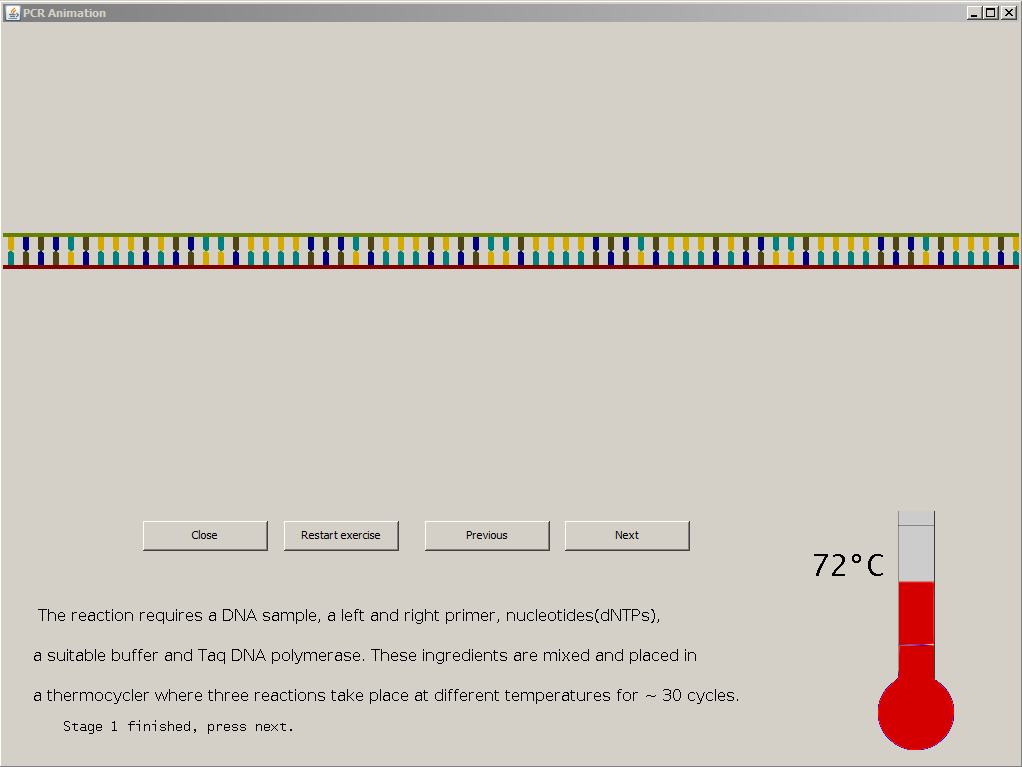
\includegraphics[width=0.7\textwidth]{./img/AnimImpl/Stage1.png}
    \caption{
      \label{fig:AnimImpl:stage1}
      Animation, Stage 1
    }
  \end{center}
\end{figure}
\end{frame}


\begin{frame}
In stage 2, Melting and Annealing, the strands are separated and the primers bind to them, with the temperature level varying accordingly.

\begin{figure}[!t]
  \begin{center}
	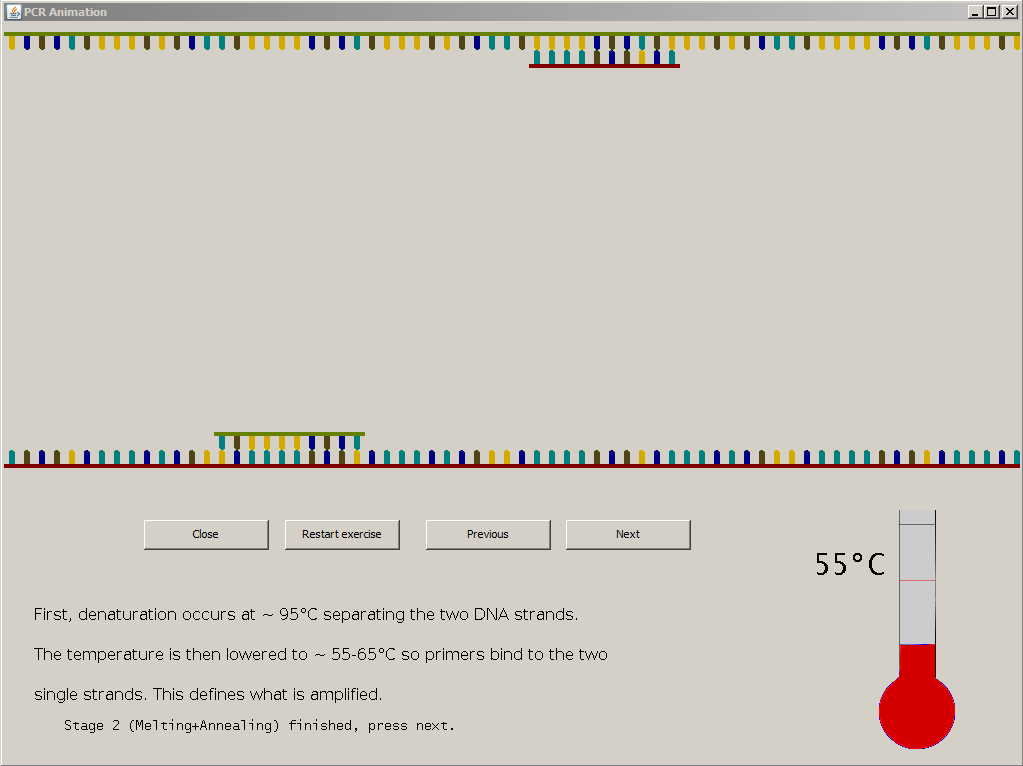
\includegraphics[width=0.7\textwidth]{./img/AnimImpl/Stage2.png}
    \caption{
      \label{fig:AnimImpl:stage2}
      Animation, Stage 2
    }
  \end{center}
\end{figure}
\end{frame}

\begin{frame}
In stage 3, Adding nucleotides, the taq polymerase creates a complementary copy of each strand, with the temperature once again raised to 72\degree C.

\begin{figure}[!t]
  \begin{center}
	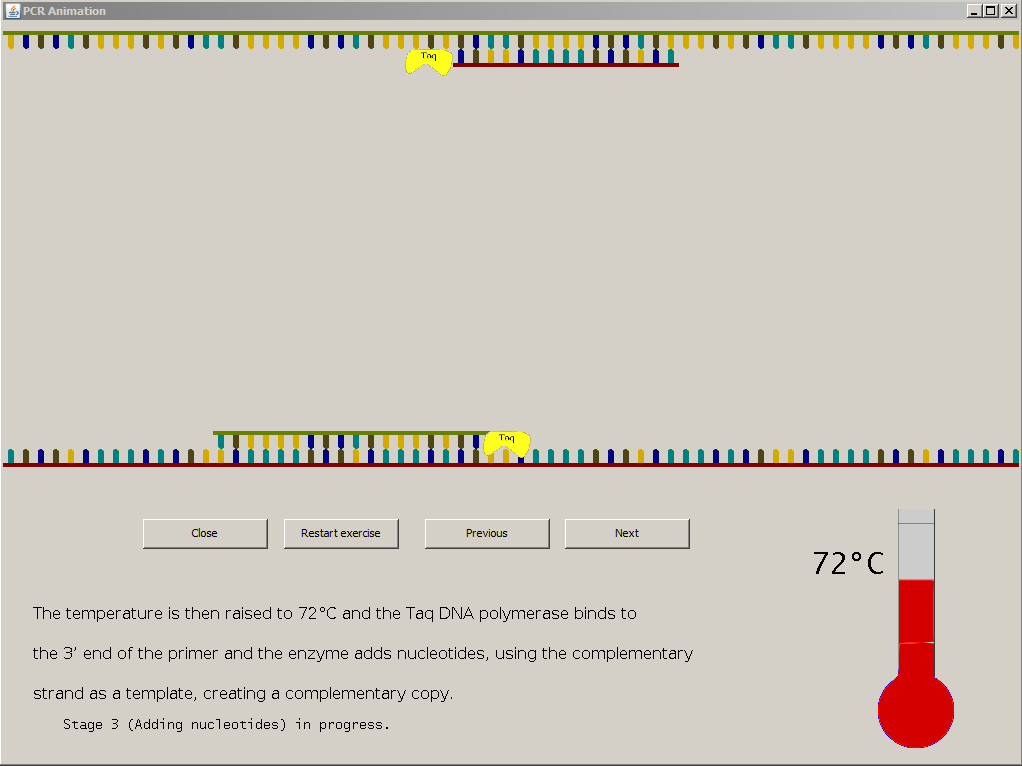
\includegraphics[width=0.7\textwidth]{./img/AnimImpl/Stage3.png}
    \caption{
      \label{fig:AnimImpl:stage3}
      Animation, Stage 3
    }
  \end{center}
\end{figure}
\end{frame}

\begin{frame}

In stages 4 and 5 another cycle of PCR is shown and the required sequence is generated for the first time.

\begin{figure}[!t]
  \begin{center}
	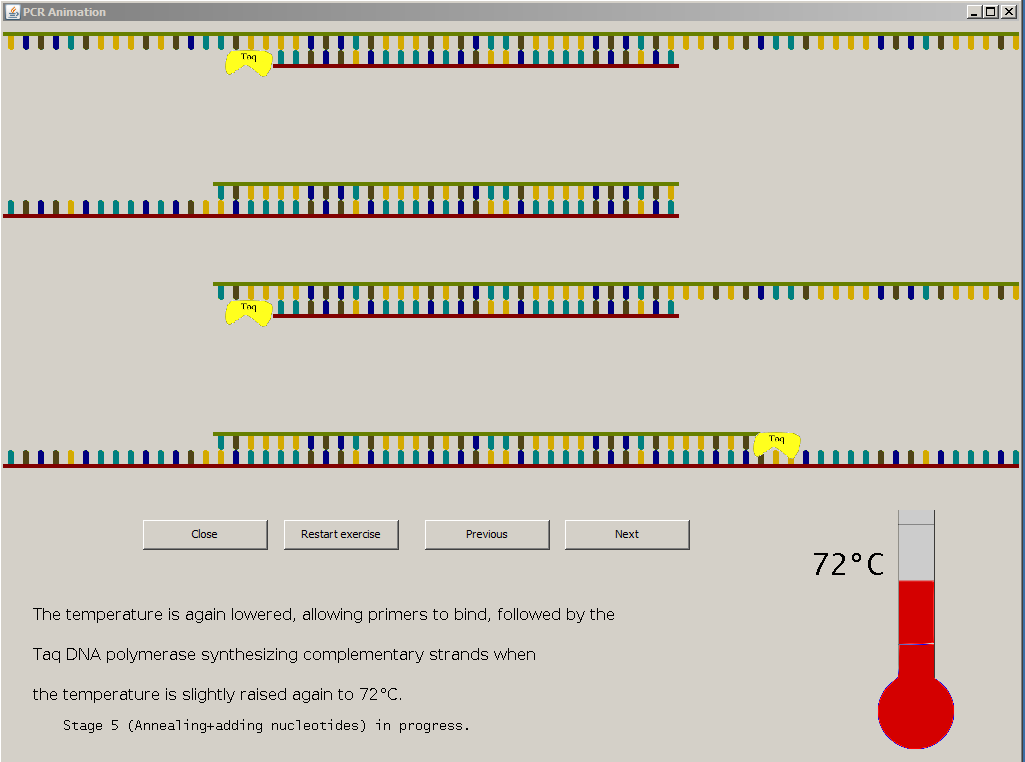
\includegraphics[width=0.7\textwidth]{./img/AnimImpl/Stage5.png}
    \caption{
      \label{fig:AnimImpl:stage5}
      Animation, Stage 5
    }
  \end{center}
\end{figure}
\end{frame}

\begin{frame}
Finally, the last two stages explain how many copies of the target sequence is produced in subsequent cycles and the user is explained that they completed the exercise and thanked for participation.

\begin{figure}[!t]
  \begin{center}
	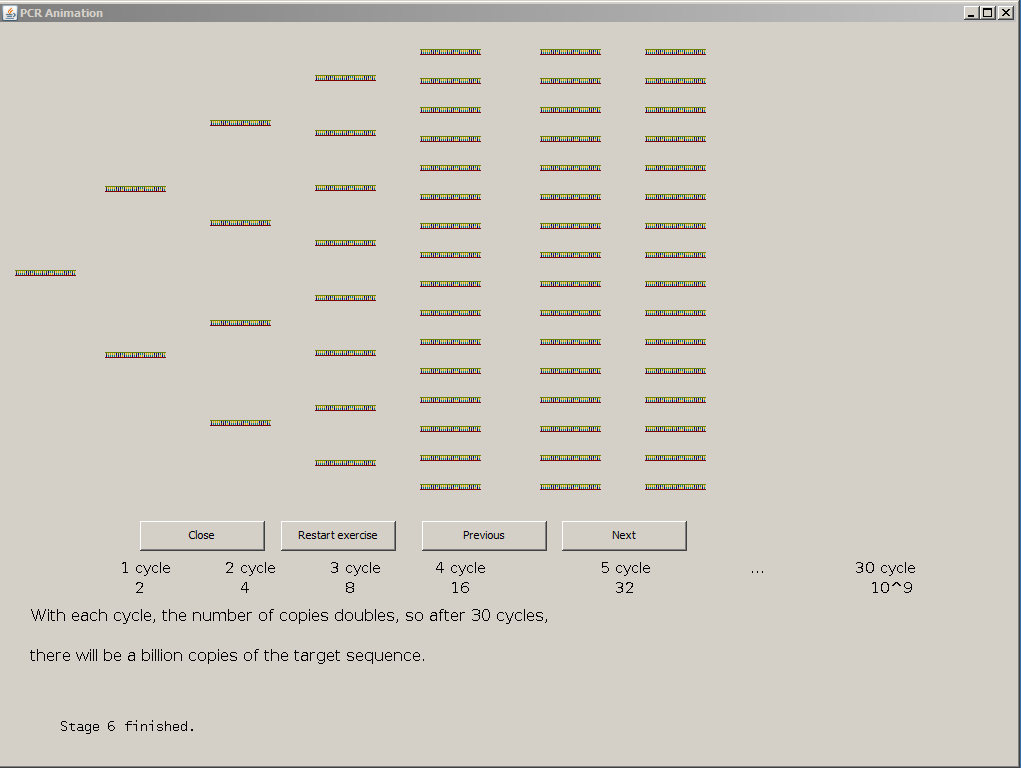
\includegraphics[width=0.7\textwidth]{./img/AnimImpl/Stage6.png}
    \caption{
      \label{fig:AnimImpl:stage6}
      Animation, Stage 6
    }
  \end{center}
\end{figure}
\end{frame}
